\chapter{Materials and Methods}


\section{Materials}


\subsection{Main component list}
\begin{enumerate}
	\item   Arduino-UNO-Wifi-Rev2: an upgraded version of the standard Arduino Uno board that incorporates several additional features to enhance its functionality.
	In this project, the onboard Wi-Fi module was fully used to provide a wireless communication.
	\item   Grove IMU 9DOF (ICM20600+AK09918): an inertial measurement unit module that integrates three sensors, including an accelerometer, gyroscope, and magnetometer.
	However, this module does not have the function of temperature compensation.
	Additionally, the chip ICM20600 only supports configuring two kinds of IIC addresses.
	Relevant datasheet is shown in Appendix~\ref{fig:limited-IIC-address}.
	\item   Gravity I2C Multiplexer: a powerful module that allows for the expansion of the I2C bus on Arduino.
	It solves the problem of overlapping IIC address.
	\item   Multi-core screened cable: to ensure the quality of wired communication.
	\item   TP-Link AC1200 Wireless Dual Band Router: to provide a local area network.
	\item   Velcro Brand Adjustable Straps, 25mm x 680mm.
	\item   18650 2,600mAh Lithium Rechargeable Batteries.
\end{enumerate}


\subsection{Software}
\begin{enumerate}
	\item JetBrains CLion: for socket server programming;
	\item Arduino IDE \& PlatformIO: for Arduino programming;
	\item Autodesk Fusion 360 \& SolidWorks \& SketchUp: for creating 3D models;
	\item Three.js: for front-end programming;
\end{enumerate}


\section{Methods}


\subsection{Arduino: data collection}\label{subsec:data-fetching}
\begin{enumerate}
%todo: refine this part
	\item   Firstly, connect the VCC pin of the I2C multiplexer to the 5V pin of the Arduino.Connect the GND pin of the multiplexer to the GND pin of the Arduino.Connect the SDA and SCL pins of the multiplexer to the SDA (A4) and SCL (A5) pins of the Arduino, respectively.Connect each IMU to one of the I2C multiplexer channels using VCC, GND, SDA, and SCL pins.
	\item   Install the required libraries for your specific IMU. For instance, the ``ICM 20600.h'', ``DFRobot\_I2C\_Multiplexer.h'', ``Wire.h” and ``MahonyAHRS.h'' libraries.
	The Attitude and Heading Reference System (AHRS) library is a set of algorithms for estimating the attitude and orientation of objects in three-dimensional space.
	These libraries are based primarily on IMU data such as the output of accelerometers, gyroscopes and magnetometers.
	The AHRS library includes one or more fusion algorithms, such as Kalman filter, Madgwick filter and Mahony filter, which fuse multiple sensor data of IMUs together to obtain more accurate, stable and reliable attitude information.
	In the experiment, we choose to use Mahony filter, which is a popular sensor fusion algorithm.
	Mahony filter combines the data of accelerometer, gyroscope and magnetometer to realize real-time estimation of the attitude and direction of objects in three-dimensional space.
	Its advantage lies in its higher computational efficiency. There is one big advantage.
\end{enumerate}


\subsection{Arduino: wireless communication} \label{subsec:5g-network}
\begin{enumerate}
	\item   To enable the built-in Wi-Fi module on Arduino-UNO-Wifi-Rev2, an external library called WiFiNINA was chosen and implemented.
	This library, provided by the official Arduino website, facilitates communication between the microcontroller and the onboard Wi-Fi module through a Serial Peripheral Interface (SPI).
	It also provides some simple examples for studying.
	\item   Initially, the Arduino was connected to a 2.4G network and attempted to establish a connection with a remote server through a handshake process.
	These functions are all included in the library and have been implemented in the kernel.
	\item   Next, a simple const string message was written to one of the Arduino's sockets and sent by the kernel.
	Given that the server was capable of printing any incoming message, the message was finally displayed on the server's console as intended.
	\item   Following this, a stress test was conducted to evaluate the system's capacity to handle a high volume of data.
	This was accomplished by continuously sending an increasing number to the server, which was then printed by the server.
	Meanwhile, the Arduino would also print out the message sent through a serial communication to the computer.
\end{enumerate}


\subsection{Socket server}
\begin{enumerate}
	\item   Based on an example sketch from an online book~\cite{beej-guide}, a simple C\texttt{++} socket server was built to support responding basic HTTP-GET requests.
	\item   Additionally, a multi thread was added to asynchronously save the motion data sent from Arduino.
	\item   To enhance the transmission of motion data to front-end users, a custom JSON encoder was developed to package the raw motion data into a compact and efficient JSON format as List~\ref{lst:json} shows.
	To increase communication rate, the content in such format has been extremely reduced by using abbreviations, where ``L\_F'' represents the motion data of left femur.
	The Euler angles were also abbreviated to ``y'', ``r'', and ``p''.
\end{enumerate}

\lstset{
	language=json,
	numbers=left,
	firstnumber=1
}
\begin{lstlisting}[caption={JSON code sent to front-end client.},label={lst:json}]
{
	"L_F": [{
		"y": -0.01,
		"r": 1.82,
		"p": -0.52}],
	"R_F": [{
		...
}
\end{lstlisting}


\subsection{Displaying engine}

With the tutorial given by official three.js website, a simple static 3D model generator was implemented.
However, such generator was not flexible enough to rapidly create a specific model, such as humans or birds.
Hence, a function that can generate models according to user customization was developed.
It works like a text operator and user could change his text to modify a corresponding model subsequently.
Relevant results are presented in the next chapter.
In the meantime, the following are the main features of this displaying engine:

%-----------This is a FIGURE-----------------------
\begin{figure}[htbp]
	\centering
	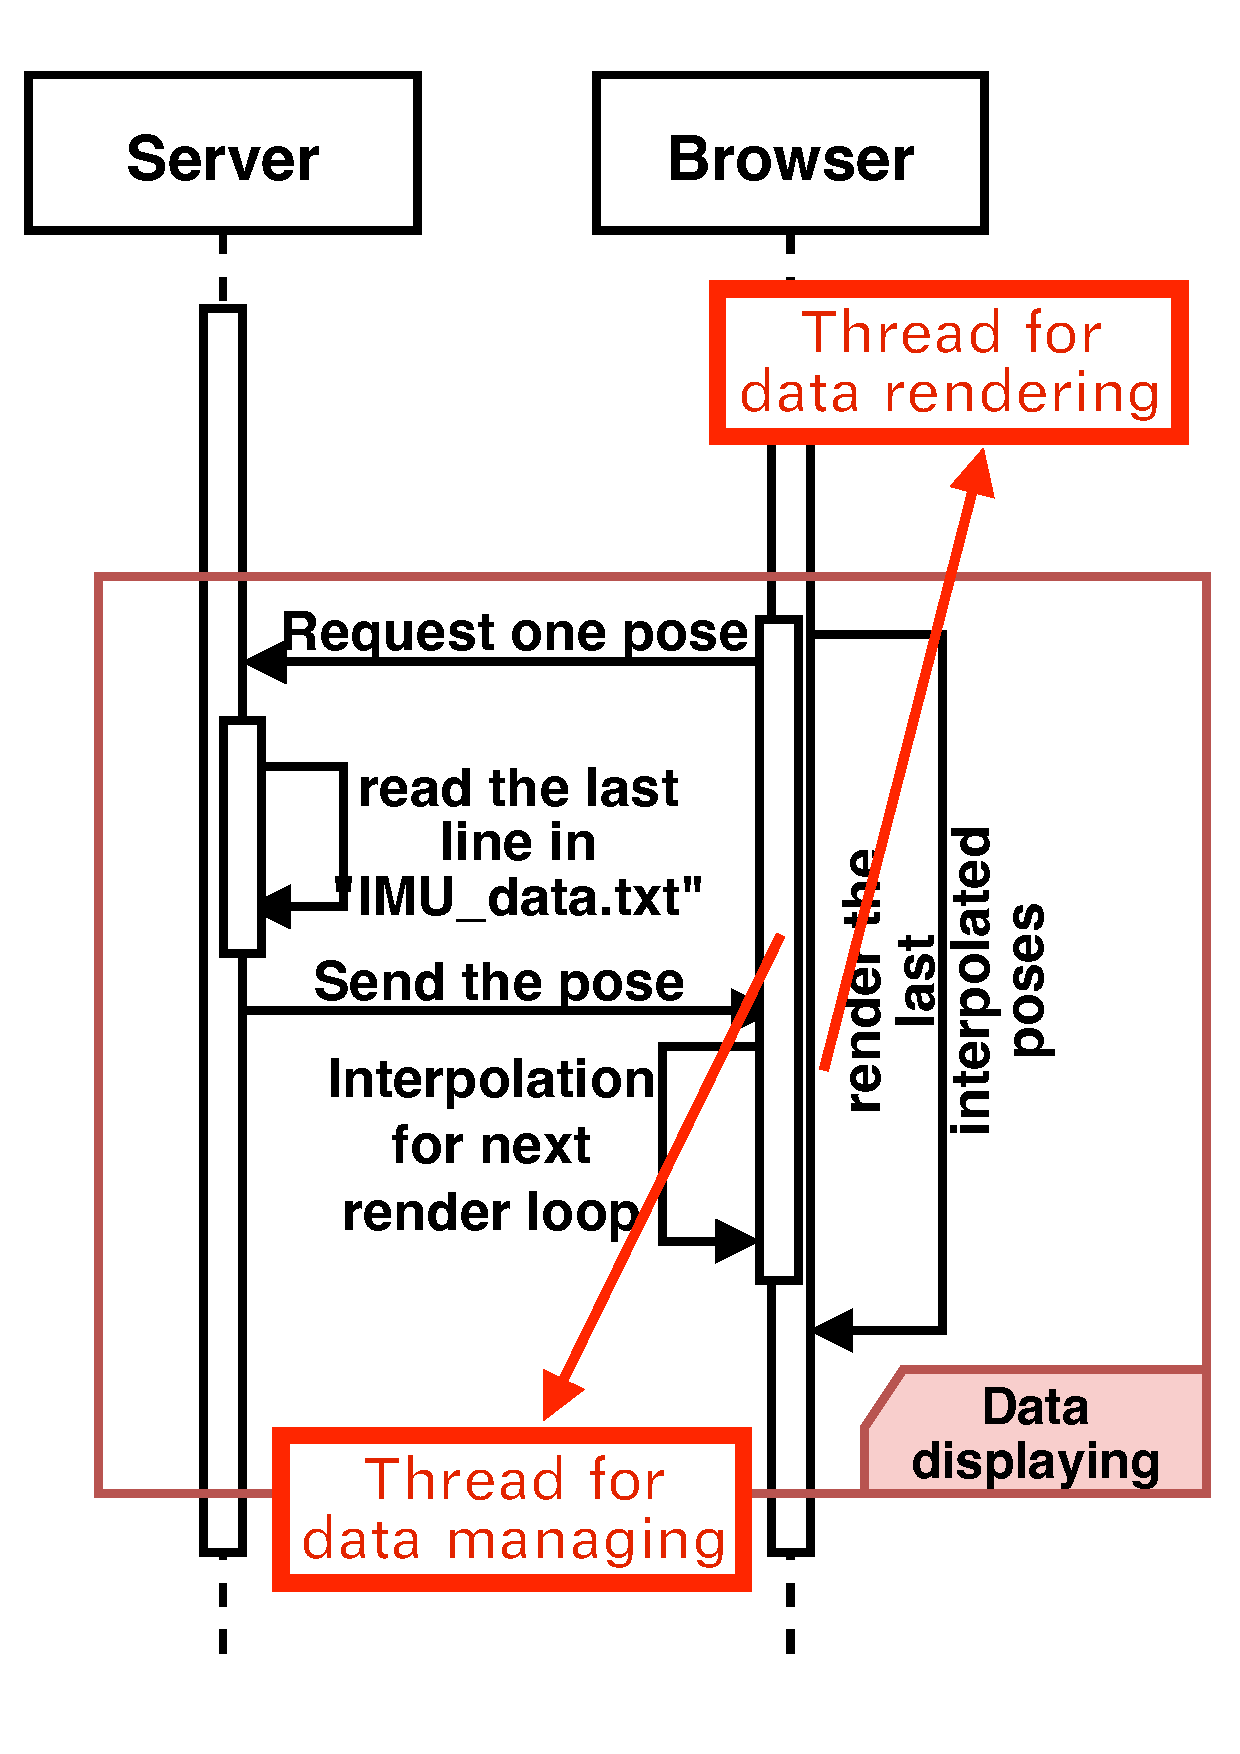
\includegraphics[width=0.5\textwidth]{
		fileForWriting/browser_sequence}
	\caption[Sequence diagram of the displaying engine]{Sequence diagram of the displaying engine.}
	\label{fig:browser_sequence}
\end{figure}
%--------End of this FIGURE -----------


\subsubsection{Reduce latency: multi-thread}
To fully achieve the goal of real time rendering, as Figure~\ref{fig:browser_sequence} may illustrate, a multi-thread method was also developed.
Particularly, one thread is designed to render the animation, inputting motion data to the model.
Simultaneously, another thread is responsible for managing motion data, requesting them from server and applying interpolation.

By achieving these, the latency raised by data fetching would be reduced to some extent.
Relevant results are shown in the next chapter and core code is shown in
Appendix~\ref{lst:flexible-input}.


\subsubsection{Reduce latency: frame interpolation}
To smooth the animation and increase frame rate, a frame interpolation function was also integrated in the thread of data managing.
For example, it would linearly insert five frames into the original single frame.
Relevant core code is shown in Appendix~\ref{lst:intorpolation-with-data-matching}.


\subsubsection{Data mapping}
To account for the mismatch between the coordinate system used in the engine and the IMU coordinate system in the real world, a mathematical mapping was also implemented to convert IMU data into angle change values for the animation.

Specifically, for the femur's up and down movements in the engine, the corresponding pitch angle is given by ±(90° + IMU pitch angle), where the positive or negative sign depends on whether the current angle is lifting the leg forward or backward.

During testing, it was observed that the roll output for the femur IMU is usually around 0° when lifting the leg forward, and around 180° when lifting the leg backward.

Given that the yaw data was unstable and useless, the current engine could only achieve the motion follow in vertical plane.
Therefore, a conditional statement using only roll data was added to the program to simply determine whether the leg is being lifted forward or backward.

Relevant core code is shown in Appendix~\ref{lst:intorpolation-with-data-matching}, including the data matching for tibia IMU\@.
The logic for tibia IMU is similar but only added its corresponding femur IMU data.
This is because the tibia part in the engine was built from its femur.

\subsubsection{Avoid jittering}
During actual testing, it was found that the model would exhibit some jittering even when the human object was freezing.
Therefore, a threshold limitation feature was added.
Only when the original data's variation exceeds a certain value, the new motion data will be regarded as valid and later input into the model.
Relevant code is shown in Appendix~\ref{lst:intorpolation-with-data-matching}.



